\section{The Hybrid Eulerian-Lagrangian Solver for the Vlasov system}
\label{sec:vlasov}
Consider the  delta $f$ form of Vlasov system in equation (\ref{eq.Vlasov}). The evolution of  perturbed distribution function $\delta f(\vartheta,\mathcal{J};\xi,\Omega;s,t)$ is
\begin{equation}\label{eq.deltaf}
    \frac{\partial \delta f}{\partial t}+ \frac{d s_{}}{d t} \frac{\partial \delta f}{\partial s_{}} + \left[\delta f, H\right]_{\vartheta,\mathcal{J}} +  \left[\delta f, H\right]_{\xi,\Omega} = \mathcal{S}~,
\end{equation}
where the   Poisson brackets are defined as
\begin{equation}
    [f,~g]_{x,y} = \frac{\partial f}{\partial x}\frac{\partial g}{\partial y}-\frac{\partial f}{\partial y}\frac{\partial g}{\partial x}~.
\end{equation}
Here $\xi,\Omega$ and $\vartheta,\mathcal{J}$ are the canonical variables corresponding to the fast  and slowly varying scales, respectively.
The source term $\mathcal{S}= -\left[f_0, \delta H\right]_{\vartheta, \mathcal{J}} - \left[f_0, \delta H\right]_{\xi, \Omega}$ 
where $f_0$ is the equilibrium distribution function and $\delta H$ denotes the perturbed Hamiltonian due to the resonant wave-particle interactions.
Note that the derivatives of $\delta H$ with respect to the slowly varying coordinates $\vartheta$ and $\mathcal{J}$ can be neglected due to the separation  of perturbation and equilibrium scales
and $\partial f_0/\partial \xi=0$ 
%is usually vanished 
since the equilibrium distribution function does not generally depend on the fast varying angle coordinate $\xi$.
Thus, the source term can be simplified as 
\begin{equation}
     \mathcal{S} = \frac{\partial \delta H}{\partial \xi}\frac{\partial f_0}{\partial \Omega}.
     %\left[f_0, \delta H\right]_{\vartheta, \mathcal{J}} + \left[f_0, \delta H\right]_{\xi, \Omega}
\end{equation}
%detailed physical meanning is not need, just clarify the fast and slow scale
%Note that, follows our
In the Hamiltonian theory for the chorus wave frequency chirping, 
the variation of the angle coordinate $\vartheta$  is proportional to the background inhomogeneity 
%Thus,  the variation of  $\vartheta$ is  small for the weakly inhomogeneous case.
and
 the dynamics of $\mathcal{J}$, $\Omega$ and $\xi$ 
 does not  depend on  $\vartheta$.  
%Since the system is $\vartheta$-free, 
Therefore we neglect the term $ \dot{\vartheta} $ in the Vlasov equation and the  Poisson bracket becomes
%evolution of the  $\vartheta$ with 
\begin{equation}
\left[\delta f, H\right]_{\vartheta,\mathcal{J}}\simeq 
 -\dot{\mathcal{J}} \frac{\partial \delta f}{\partial \mathcal{J}}      
\end{equation}
where the dot denotes the time derivative.

We now apply the hybrid method to the Vlasov system where the fast and slowly varying scales have been separated in the  Hamiltonian theory.
%But unlike the manipulations applied in a conservative HLE method \cite{shiroto2022} which solves the advection equations of shape functions unlike particle-in-cell method on configuration domain and model the velocity by discrete super-particles, 
We model the fast varying  phase space $\xi,\Omega$ by Eulerian method and model the slowly varying coordinate
$\mathcal{J}$ 
and the resonance frame  coordinate $s$ through Lagrangian method.
The 
%Klimontovich description-like 
distribution function is written as \cite{shiroto2022}
\begin{equation}
    \delta f(\xi,\Omega,\mathcal{J},s,t) = \sum_{k,l} g_{k,l}(t,\xi,\Omega)\delta(s-s_k(t),\mathcal{J}-\mathcal{J}_l)~,
\end{equation}
where $g_{k,l}(t,\xi,\Omega)$ is the distribution function in $\xi,\Omega$ space with $k$ and $l$ the index of the Lagrangian marker.
% the  delta function represents the markers in  space $s_k$, and $\mathcal{J}_l$ with .
Then the evolution equation for $g_{k,l}(t,\xi,\Omega)$ for each marker labeled by $k$ and $l$ is
%of the HLE method
\begin{equation}\label{eq.Euler}
\frac{\partial g}{\partial t} + \left[g,H\right]_{\xi,\Omega} = \mathcal{S}~.
\end{equation}
Here we omit the index $k$ and $l$ for $g$ for convenience.
For the Lagrangian step, the marker is required to move with the resonance frame on the spatial domain   
\begin{equation}\label{eq.resonance}
        \dot{s}_k = v_r(s_k(t))~,
\end{equation}
where $v_r$ is  the  resonant velocity.
 %Since the dynamics of momentum $\mathcal{J}$ is fully decoupled with $\xi,~\Omega$,
The motion equation for slowly varying coordinate $\mathcal{J}$ is
% \begin{equation}
%     \begin{aligned}
%         \dot{\vartheta} &= \frac{\iint \mathcal{F}_i(t,\xi,\Omega)\left[\vartheta,H\right]_{\vartheta,\mathcal{J}} \mathrm{d}\xi\mathrm{d}\Omega}{\iint \mathcal{F}_i(t,\xi,\Omega)\mathrm{d}\xi\mathrm{d}\Omega}~,\\
%         \dot{\mathcal{J}} &= \frac{\iint \mathcal{F}_i(t,\xi,\Omega)\left[\mathcal{J},H\right]_{\vartheta,\mathcal{J}} \mathrm{d}\xi\mathrm{d}\Omega}{\iint \mathcal{F}_i(t,\xi,\Omega)\mathrm{d}\xi\mathrm{d}\Omega}~.\\
%     \end{aligned}
% \end{equation}
% Note that, follows our Hamiltonian theory \cite{}, the variation of $\vartheta$ coordinate is proportional to the background inhomogeneity. Thus, for the weakly inhomogeneous case, the variation of the angle coordinate $\vartheta$ is considerably small.
% Besides, the dynamics of $J$, $\Omega$ and $\xi$ are also independent on $\vartheta$, i.e., the system is $\vartheta$-free, and we can neglect the evolution of $\vartheta$. 
% Moreover, the dynamics of momentum $\mathcal{J}$ is fully decoupled with $\xi,~\Omega$ dimension, thus the integration over the fast varying dimension can be eliminated, and the force equations in our simulation scheme are
\begin{equation}
    \begin{aligned}\label{eq.Lagrangian}
        \dot{\mathcal{J}} &= \left[\mathcal{J},H\right]_{\vartheta,\mathcal{J}}~.
    \end{aligned}
\end{equation}

\subsection{The Eulerian step}
Now we solve the fast-varying phase space dynamics for each Lagrangian at $s_k,\mathcal{J}_l$.
For the numerical treatment, the Vlasov equation (\ref{eq.Euler}) is expressed as
\begin{equation}\label{eq.Euler2}
    \frac{\partial g}{\partial t} + m \frac{\partial  g}{\partial \xi} - n \frac{\partial  g}{\partial \Omega}= \mathcal{S}~,
\end{equation}
where 
%$g \equiv \mathcal{F}_i$ and 
%we use $m$, $n$ to represent the derivatives of the Hamiltonian
\begin{equation}
        m(\xi,\Omega) = \frac{\partial H}{\partial \Omega},~ n(\xi,\Omega) = \frac{\partial H}{\partial \xi}~.
\end{equation}
%The partial differential equation is a typical form of , and 
To achieve high-order accuracy, we apply the IDO method \cite{imadera2009} to solve the 2D Vlasov equation in $\xi,\Omega$ domain.
The IDO scheme applies the polynomial as local interpolation functions to replace the distributions along each coordinate in phase space. 
%The differential and integral in the advection parts of the Vlasov equation can be then analytically calculated. 
Here
%, we present a second-order scheme to demonstrate the basic routines. 
a second-order  polynomial is used as interpolation stencil for a function $g(x)$ from $x_i$ to $x_{i+1}$,
\begin{equation}\label{eq.intg}
    G(x,g_{i},g_{i+1},\sigma_{i+\frac{1}{2}}) = a\left(x-x_i\right)^2+b\left(x-x_i\right)+c~,
\end{equation}
where $g_i \equiv g(x_i)$, $g_{i+1} \equiv g(x_{i+1})$ are function values on the grid, and $\sigma_{i+\frac{1}{2}}$ is the cell integral value 
\begin{equation}
    \sigma_{i+\frac{1}{2}} \equiv \int_{x_i}^{x_{i+1}} g(x)~\mathrm{d}x~,
\end{equation}
and the coefficients are determined and from the grid value and the line integral over the cell,
\begin{equation}
    \begin{aligned}
        a & =\frac{3\left(g_i+g_{i+1}\right)}{\Delta x^2}-\frac{6 \sigma_{i+\frac{1}{2}}}{\Delta x^3}~, \\
        b & =-\frac{2\left(2 g_i+g_{i+1}\right)}{\Delta x}+\frac{6 \sigma_{i+\frac{1}{2}}}{\Delta x^2}~, \\
        c & = g_i~.
    \end{aligned}
\end{equation}

For equation (\ref{eq.Euler2}), the derivatives of $g$ with respect to $\xi$ and $\Omega$ are numerically represented by the interpolating stencil introduced above. 
The discretized form of the Vlasov equation becomes,
\begin{equation}\label{eq.disV}
    \begin{aligned}
    \left.\frac{\partial g}{\partial t}\right|_{i,j}   & =  - m_{i,j} \left.\frac{\partial}{\partial \xi} G\left(\xi;g_{i,j},g_{i+1,j},\rho_{i+\frac{1}{2},j}\right)\right|_{i,j} 
    \\
    & + n_{i,j}  \left.\frac{\partial}{\partial \Omega}G\left(\Omega;g_{i,j},g_{i,j+1},\kappa_{i,j+\frac{1}{2}}\right)\right|_{i,j}
    \\
    & +  \mathcal{S}_{i,j}~,
    \end{aligned}
\end{equation}
where $i$ and $j$ are the grid index for $\xi$ and $\Omega$, respectively. 
 %$g_\xi$ and $ g_\Omega$ denote the derivatives along $\xi$ and $\Omega$ directions, 
%The stencil is applied along both $\xi$ and $\Omega$ dimensions. 
The grid and the sampling points are demonstrated in Fig.~\ref{fig.grids}.
\begin{figure}[htbp]
    \centering
    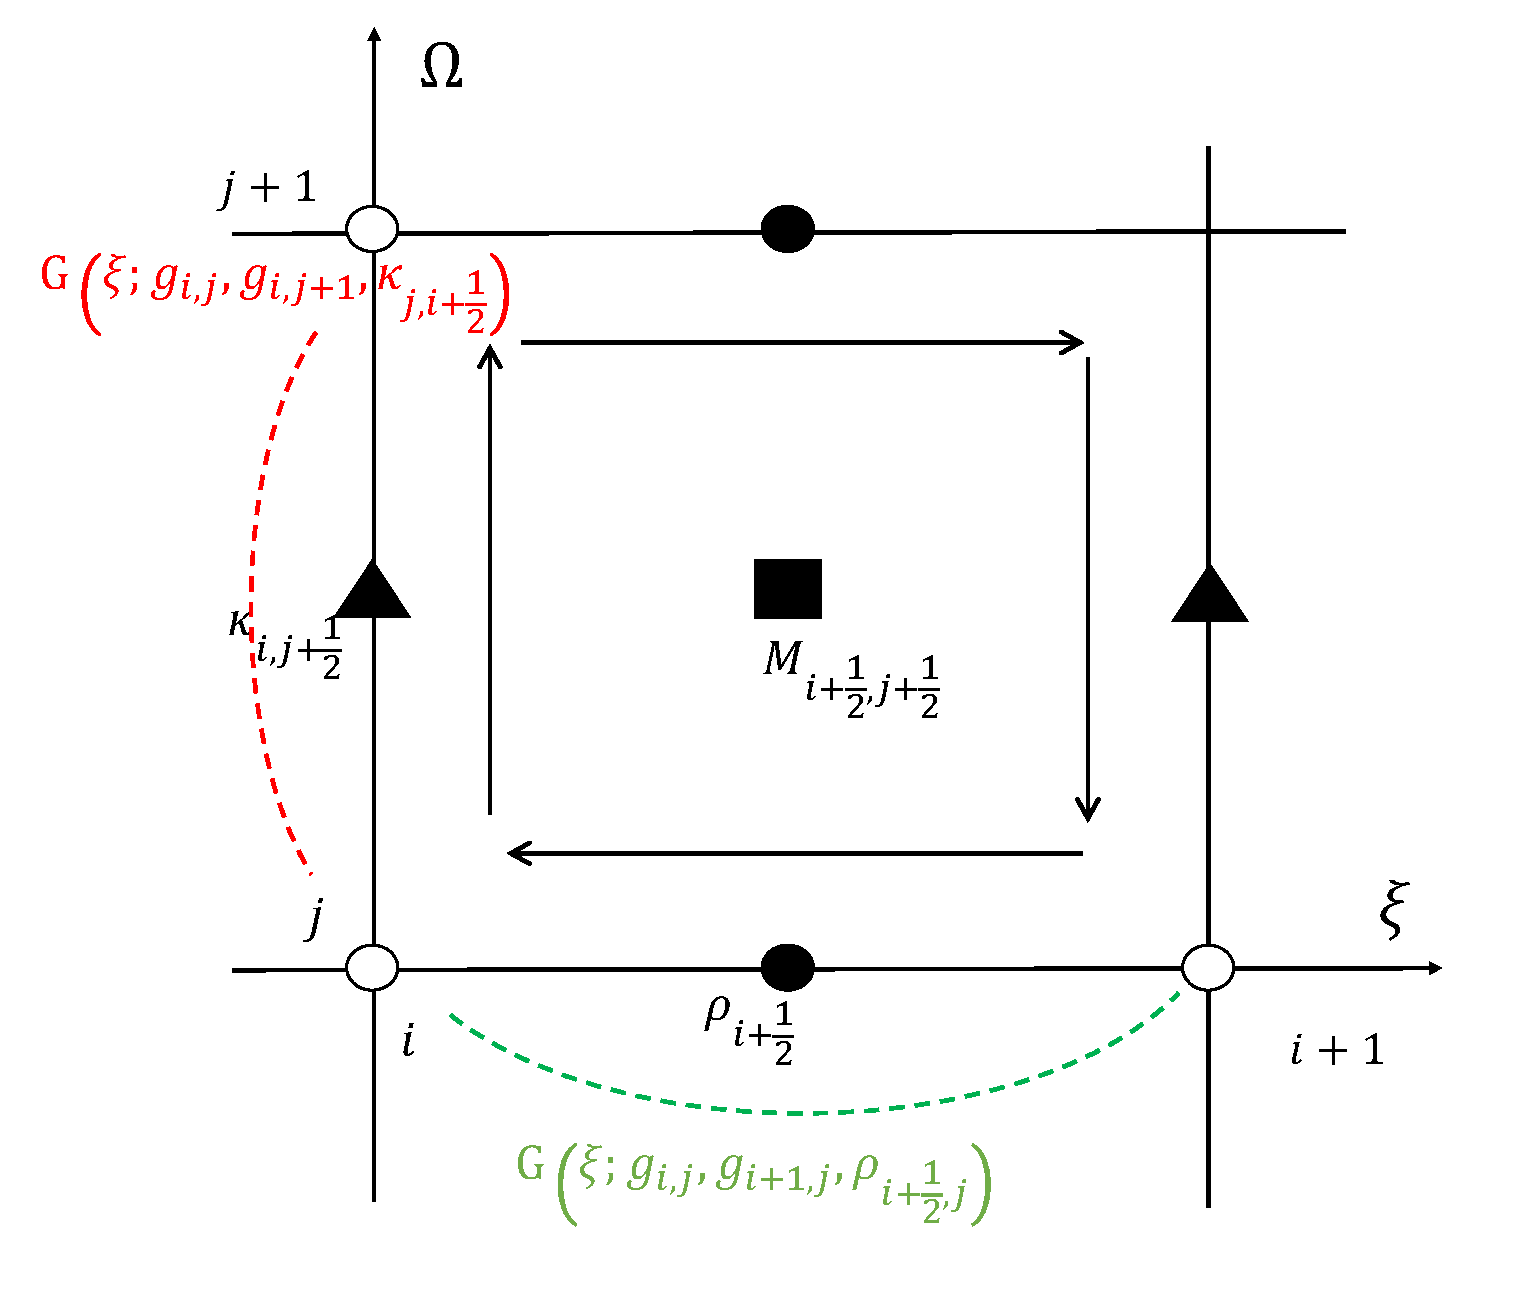
\includegraphics[scale=0.3]{cpc_img/IDO.pdf}
    \caption{The interpolating functions and cell integrated values in $\xi,\Omega$ domain.}
    \label{fig.grids}
\end{figure}
%middle step 1, construct f(xi) and f(Omega)
%Firstly, we construct interpolation function according to the stencil to replace $f$ along $\xi$ and $\Omega$ directions and calculate the derivatives on the $i,j$ grid as
%Applying the interpolation function $G$ defined in Eq.~(\ref{eq.intg})  along $\xi$ and $\Omega$  yields the derivatives
% Then the derivatives are given by 
%\begin{equation}
%    \begin{aligned}
%    \frac{\partial g_{i,j}}{\partial \xi}
%         \simeq \left. \frac{\partial}{\partial \xi} G\left(\xi;g_{i,j},g_{i+1,j},\rho_{i+\frac{1}{2},j}\right)\right|_{i,j}~, \\
%         \frac{\partial g_{i,j}}{\partial \Omega}
% \simeq \left.\frac{\partial}{\partial \Omega}G\left(\Omega;g_{i,j},g_{i,j+1},\kappa_{i,j+\frac{1}{2}}\right)\right|_{i,j}~,
%    \end{aligned}
%\end{equation}

The interpolation relies on the line integrated values $\rho_{i+\frac{1}{2},j}=\int_{\xi_i}^{\xi_{i+1}}g_{j}(\xi)\mathrm{d}\xi$ and $\kappa_{i,j+\frac{1}{2}}=\int_{\Omega_j}^{\Omega_{j+1}}g_{i}(\Omega)\mathrm{d}\Omega$.
%The calculation at this step relies upon $\rho_{i+\frac{1}{2},j}$ and $\kappa_{i,j+\frac{1}{2}}$, which are the line integrated value of $\mathcal{F}$ 
To solve the integral value $\rho$ and $\kappa$, we consider the Eq.~(\ref{eq.Euler2}) on given $j$ and $i$ grid respectively, and integrate it along $\xi$ and $\Omega$ over the grid interval, which yields the time evolution of the integral values
%, accroding to the definition in Eq.~(\ref{eq.intg}). The time evolution of the integral value is derived from the Vlasov equation,
\begin{equation}\label{eq.line}
    \begin{aligned}
    \left.\frac{\partial \rho}{\partial t}\right|_{i+\frac{1}{2},j} &= \int_{\xi_i}^{\xi_{i+1}}[ - m_j(\xi) \left.\frac{\partial g}{\partial \xi}\right|_{j}(\xi) + n_j(\xi) \left.\frac{\partial g}{\partial \Omega}\right|_{j}(\xi) + \mathcal{S}_j(\xi)]~\mathrm{d} \xi
    \\
    \left.\frac{\partial \kappa}{\partial t}\right|_{i,j+\frac{1}{2}}
    &= \int_{\Omega_j}^{\Omega_{j+1}}[ - m_i(\Omega) \left.\frac{\partial g}{\partial \xi}\right|_{i}(\Omega) + n_i(\Omega) \left.\frac{\partial g}{\partial \Omega}\right|_{i}(\Omega) + \mathcal{S}_i(\Omega)]~\mathrm{d} \Omega
    \end{aligned}
\end{equation}
%Then, enters step 2, solve Eq.~(\ref{eq.line})
%In the above integrals on the right-hand-side, 
We apply the third-order central interpolation scheme to approximate the functions $m$ and $n$ along the $\xi$ and $\Omega$ dimension and use the interpolating stencil again to approximate the derivatives, 
\begin{equation}
    \begin{aligned}
       \left.\frac{\partial g}{\partial \xi}\right|_{j}(\xi)
        &\simeq G\left(\xi;\left.\frac{\partial g}{\partial \xi}\right|_{i,j},\left.\frac{\partial g}{\partial \xi}\right|_{i+1,j},g_{i+1,j}-g_{i,j}\right)
        \\
        \left.\frac{\partial g}{\partial \Omega}\right|_{j}(\xi)
         &\simeq G\left(\xi;\left.\frac{\partial g}{\partial \Omega}\right|_{i,j},\left.\frac{\partial g}{\partial \Omega}\right|_{i+1,j},    \left.\frac{\partial \rho}{\partial \Omega}\right|_{i+\frac{1}{2},j}\right)
         \\
         \left.\frac{\partial g}{\partial \Omega}\right|_{i}(\Omega) 
     &\simeq G\left(\Omega;\left.\frac{\partial g}{\partial \Omega}\right|_{i,j},\left.\frac{\partial g}{\partial \Omega}\right|_{i,j+1},g_{i,j+1}-g_{i,j}\right)\\
         \left.\frac{\partial g}{\partial \xi}\right|_{i}(\Omega) 
  &\simeq G\left(\Omega;\left.\frac{\partial g}{\partial \xi}\right|_{i,j},\left.\frac{\partial g}{\partial \xi}\right|_{i,j+1},\left.\frac{\partial \kappa}{\partial \xi}\right|_{i,j+\frac{1}{2}}\right)
    \end{aligned}
\end{equation}
%The interpolations bring new dependence on intergral value $\rho_{\Omega;i+\frac{1}{2},j}$ and $\kappa_{\xi;i,j+\frac{1}{2}}$. Therefore, 
We apply additional interpolation functions to approximate 
%$\rho$ along $\Omega$ and $\kappa$ along $\xi$ to calculate its 
the derivatives
\begin{equation}
    \begin{aligned}
    \left.\frac{\partial \rho}{\partial \Omega}\right|_{i+\frac{1}{2},j}
    &\simeq \left.\frac{\partial}{\partial \Omega} G(\Omega;\rho_{i+\frac{1}{2},j},\rho_{i+\frac{1}{2},j+1}, M_{i+\frac{1}{2},j+\frac{1}{2}})\right|_{i+\frac{1}{2},j}~, \\
    \left.\frac{\partial \kappa}{\partial \xi}\right|_{i,j+\frac{1}{2}}
 &\simeq \left.\frac{\partial}{\partial \xi} G(\xi;\kappa_{i,j+\frac{1}{2}},\kappa_{i+1,j+\frac{1}{2}}, M_{i+\frac{1}{2},j+\frac{1}{2}})\right|_{i,j+\frac{1}{2}}~,
    \end{aligned}
\end{equation} 
%the interpolations rely both on 
where the surface integral $M_{i+\frac{1}{2},j+\frac{1}{2}}=\int_{\xi_i}^{\xi_{i+1}}\int_{\Omega_j}^{\Omega_{j+1}}g(t,\xi,\Omega)d\xi d\Omega$.
% and it can be readily transformed to the loop integral 
The time evolution of this surface integral according to the Stokes theorem is given by
\begin{equation}\label{eq.area}
    \begin{aligned}
         \left.\frac{\partial M}{\partial t}\right|_{i+\frac{1}{2},j+\frac{1}{2}}
         &= \int_{\xi_i}^{\xi_{i+1}} n_{j+1}(\xi) g_{j+1}(\xi)~\mathrm{d}\xi - \int_{\Omega_j}^{\Omega_{j+1}} m_{i+1}(\Omega) g_{i+1} (\Omega)~\mathrm{d} \Omega \\
        & - \int_{\xi_i}^{\xi_{i+1}} n_{j}(\xi) g_{j}(\xi)~\mathrm{d}\xi + \int_{\Omega_j}^{\Omega_{j+1}} m_{i}(\Omega) g_{i} (\Omega) \mathrm{d}\Omega \\
        &+ \iint \mathcal{S}(\xi,\Omega)~\mathrm{d}\xi\mathrm{d}\Omega~.
    \end{aligned}
\end{equation}
%The line interals in above equation are then solved similarly as in Eq~(\ref{eq.line}), and the area 
Here the integral of the source term is solved by trapezoidal integration.
%The RK method
Equations (\ref{eq.disV}), (\ref{eq.line}), and (\ref{eq.area})
are a set of ordinary differential equations that can be solved  by Runge-Kutta (RK) method.
%-------------------------------%-------------------------------
%Boundary conditions
For the boundary conditions, 
%within one Lagrangian marker, the spatial grid acctually extents over several wave lengths and should contains various $F(t,\xi,\Omega)$.  When staying the resonant frame, the translation motion of the resonances is shifted to zero and the resonances sit within the reference frame. The resonanct particles are regarded as identical, so the boundary condition of 
the distribution function 
%between two neighbor resonances 
in  the resonant frame
is assumed to be periodic in the phase angle $\xi$,
\begin{equation}
    g\left(\xi,\Omega,t\right)=g\left(\xi+2 \pi,\Omega,t\right)
\end{equation}
and
%Besides, for the delta $f$ method, we manually set the momentum for the perturbed distribution, thus 
the values of the perturbed distribution vanish at the $\Omega$ boundaries.
% is simply vanished, i.e.,
% \begin{equation}
%     g\left(\Omega\right)=0~.
% \end{equation}
%Nota that, in our simulation the calculation frame is shifted to the approximate resonant frame, which uses the linear frequency and the mode number determined by the linear dispersion relation to compute the resonant velocity with no chirping. Once the frequency chirping occurs, the actual resonant velocity deviates from the calculation frame and advances the resonance in the middle of the cell eventually to move outside it, which causes the breakdown of the periodic boundary condition. During the frequency chirping, the resonance still needs to spend a finite time to move through the cell with the spreading $l$ in the approximate resonant frame, which is the time window to validate our simulation. The time window can be extended as long as the resonances are frozen in the approximate resonant frame, which is as close as the actual resonant frame. 
%For the better unstand the scheme, we breifly illustrate the simulation domain and the principle procedures of the hybrid scheme in Fig.~\ref{fig.demo}. The above numerical solution for local distribution is refereed as process A in Fig.~\ref{fig.demo}.
\begin{figure}[htbp]
    \centering
    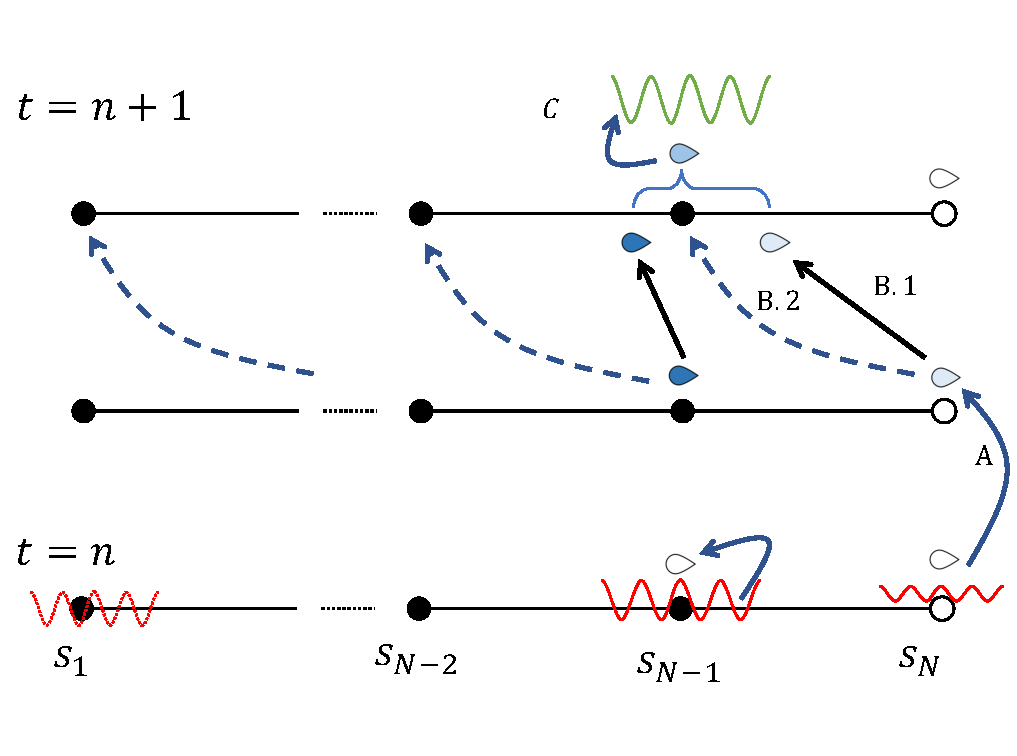
\includegraphics[scale=0.5]{cpc_img/Hybrid_demo.pdf}
    \caption{Schematic illustration of the hybrid Vlasov simulation scheme.}
    \label{fig.demo}
\end{figure}

\subsection{The Lagrangian step}
%After evolving the perturbed distribution on the $\xi-\Omega$ grids, 
%to solve the rest part of the Vlasov equation (\ref{eq.deltaf}) with respect to $s_i, \mathcal{J}$,
For the Lagrangian markers,
%with label $l$ for the coordinate $ \mathcal{J}$, 
%without the calculation for $\vartheta$, we sample the markers at $s$ and $\mathcal{J}$ dimension.
% We use $N_s$ points for sampling $s$, and use $N_\mathcal{J}$ sampling points in $\mathcal{J}$ dimension for each $s_i$. 
% Thus, the binary index $(i,j)$ is used to denote the marker, and the total number of the Lagrangian markers is $N_s \times N_\mathcal{J}$.
% On the $s$ dimension, $N_s$ is equal to $N_g$, the number of the grids used to discretize the wave equation, and the markers are initially set one to one onto the fixed wave grids $s_g$.
%Sampling of J
the sampling point for $\mathcal{J}$ is chosen to ensure  a uniform sampling to the initial equilibrium distribution,
%is used to sample the $\mathcal{J}$ coordinate
%function,
% at a given $s$, 
\begin{equation}
    f_0(\mathcal{J}) = l/N_l, 
    %~ j = 1, N_\mathcal{J}~,
\end{equation}
where $N_l$ is the total number of sampling points for $\mathcal{J}$. An illustration is shown in Fig. \ref{fig.uni_grid}(a).

%Since the resonant velocity varies along the resonance frame coordinate $s$,  
%to persist the spatial alignment between Lagrangian markers and the fixed grid, we apply a nonuniform grid i.e., an initial nonuniform sampling points.To arrange the initial
For the spatial sampling of the marker, we put them initially on the fixed grid, $s_i$, the grid used to solve the wave.
To ensure that time for every marker goes through one grid is identical, we also apply nonuniform sampling, thus nonuniform wave grid.
We first calculate the transit time of a marker through the whole simulation domain
%from $s_1$ and $s_{N_g}$ denoting the two end points of the domain,
\begin{equation}
    T = \int_{s_1}^{s_N} \frac{\mathrm{d}s}{v_r(s)}~
\end{equation}
where $v_r(s)$ is the local resonant velocity that has been predetermined from the background equilibrium parameter.
Then the simulation time step is set as $\Delta t = T/N$ with $N$ the total number of sampling points/grids.
Finally the initial spatial coordinates of the markers are set according to equation (\ref{eq.resonance}) gives the trajectory of the Lagrangian marker. 
\begin{equation}
    s_{k+1} = s_k +  \int_{t}^{t+\Delta t} v_r(s_k(t)) \mathrm{d}t~
\end{equation}
where $k=1,2,3,...,N$.
The nonuniform grids with size $\Delta s$ are shown in Fig. \ref{fig.uni_grid}(b). 
%An illustration of the nonuniform is 
With such nonuniform grid, the initially sampled Lagrangian markers on the grid reach the next adjacent grid after a time interval $\Delta t$.
\begin{figure}[htbp]
    \centering
    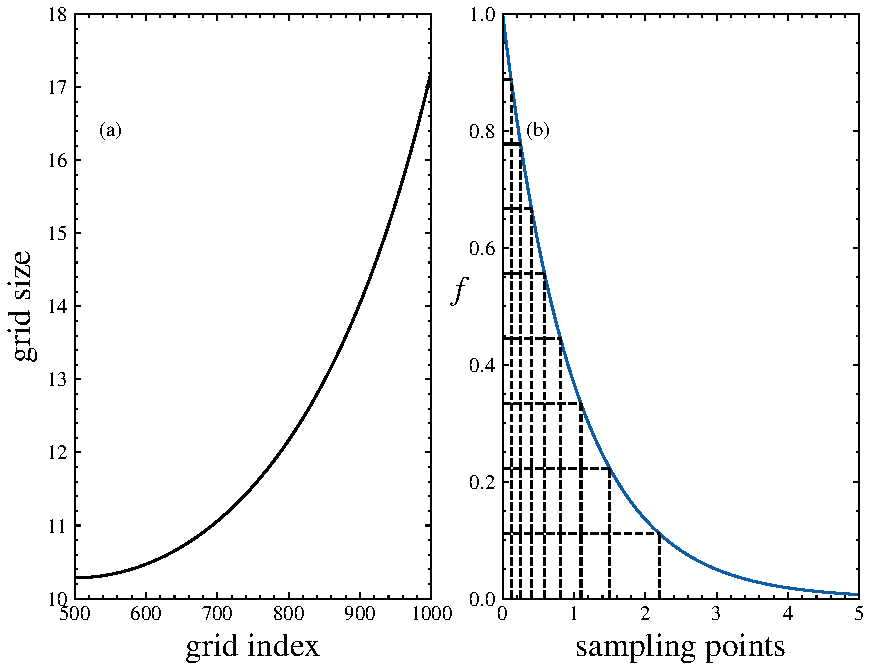
\includegraphics[scale=0.5]{cpc_img/fig_nu_grid.pdf}
    \caption{The nonuniform spatial grid obtained from resonance velocity. 
    %Here the number of grid points $N=500$.
    }
    \label{fig.uni_grid}
\end{figure}
%where $t_i = i \Delta t$.
%Push feon to new Lagrangian markers
%The trajectory for each Lagrangian marker $s_i,\mathcal{J}_j$ is determined by equations (\ref{eq.resonance}) and (\ref{eq.Lagrangian}).
%Thus the distribution $g_{k,l}(t^{n+1},\xi,\Omega)$ from the Eulerian step is pushed to the new location $s_{k+1},\mathcal{J}_l$ of the Lagrangian marker
Thus we successively push the distribution $g_{k,l}(\xi,\Omega)$  from  $s_k$ to the next grid $s_{k+1}$ for each time interval $\Delta t$.
%drop the maker which leaves the simulation zone, and set a new distribution $g(\xi,\Omega) = 0$ for which enters the simulation domain at each time iteration. In the meantime, $\mathcal{J}_j$ is updated by the Runge-Kutta (RK) method.
%, as shown in $B.2$ route. 
After pushing the Lagrangian maker from the $n^\mathrm{th}$ to the $n+1^\mathrm{th}$ time step, 
%the distribution $g(t^{n+1},\xi,\Omega)$ from the Eulerian iteration is moved to this new location $s_i^{n+1},\mathcal{J}^{n+1}_j$. 
the Hamiltonian  is re-calculated by  the  equilibrium quantities  at the new location of $s$ and $\mathcal{J}$, 
%$s_i^{n+1},\mathcal{J}^{n+1}_j$ 
which are needed for evolving the distribution in $\xi-\Omega$ space at the next time step.

We also apply the uniform grid and sampling of Lagrangian marker on $s$ to verify the nonuniform grid approach. 
After a given time step $\Delta t$ the markers deviated from the fixed grid, thus  we need to interpolate the distribution function and its derivatives required in the IDO scheme from the adjacent marker to the fixed $s$ grid.
The procedures are similar to the semi-Lagrangian method \cite{sonnendrucker1999,cottet2018}.
After interpolation, the markers realigned to the grid, and the next iteration start again from the grid location.
As shown in Fig.~\ref{fig.cmp1}, the wave amplitudes calculated from  the two approaches converge  as the smaller grid sizes are used for  the   uniform grid with interpolation.  
\begin{figure}[htbp]
    \centering
    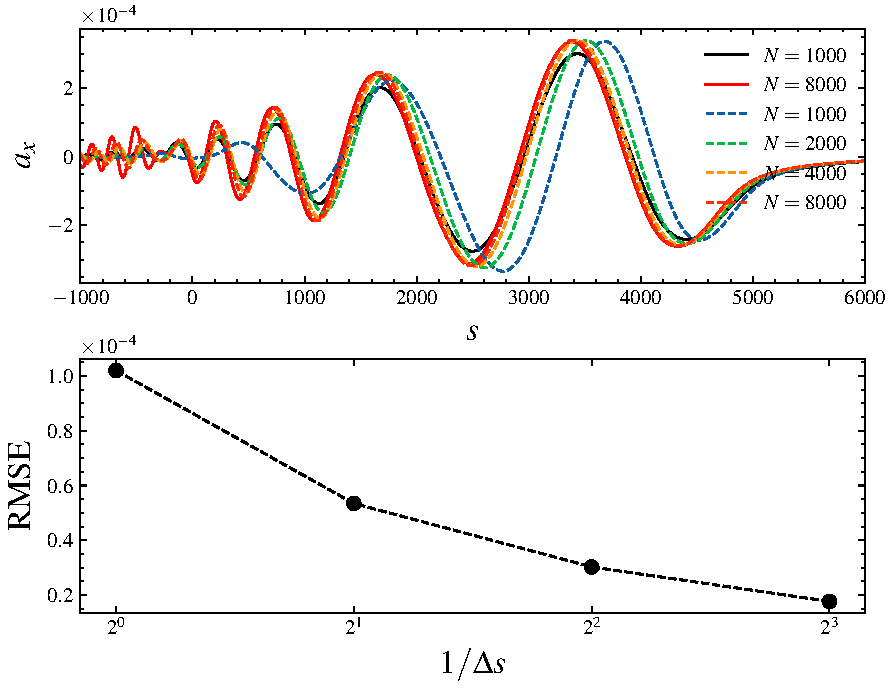
\includegraphics[scale=0.5]{cpc_img/fig_semiL.pdf}
    \caption{Wave amplitude from semi-Lagrangian method with linear interpolation of distribution at different uniform grid sizes (dashed-line) and the nonuniform grid (solid line).
    }
    \label{fig.cmp1}
\end{figure}
The evolution of $\vartheta,\mathcal{J}$ in Eq. (\ref{eq.Lagrangian}) are simply solved by applying the RK method.

Since the evolution in $\xi,\Omega$ phase space is much faster than that in the $s_i,\vartheta,\mathcal{J}$ domain,
we use the large fixed time step $\Delta t$ for the Lagrangian calculation
and  apply a much smaller time step $\Delta t_{adp}$ for solving the fast varying dynamics on the Eulerian domain. 
% Here, we apply adaptive time step RK method to solve the dynamcis within one $\Delta t$, i.e., 
Here the smaller time steps $\Delta t_{adp}$ are adaptively obtained from real time error analysis using the  adaptive time step RK method.
%of the second and the third order RK during step $A$ as shown in Fig.~\ref{fig.demo}.
Thus 
%As the time step adaptively adjust its size, within one $\Delta t$ is also dynamical, and satisfies
\begin{equation}
    \sum_{n=1}^N \Delta t_{adp}= \Delta t ~.
\end{equation}
where $N$ is the total number of iterations within one $\Delta t$. 
%The last fast scale time difference $\Delta t_{adp}$ at $N-1$ th iteraction is given by 
% \begin{equation}
%     \Delta t_{adp}^{N-1} = \Delta t - \sum_0^{N-1} \Delta t_{adp}
% \end{equation}
%We intutively visualize the time step varying during the iteraction 
As shown in Fig.~\ref{fig.adapetive}, 
%At each step within one $\Delta T$, 
$\Delta t_{adp}$ is adjusted and reduced to a smaller value to satisfy the error constraint. As the system evolves nonlinearly, 
the  time step $\Delta t_{adp}$ is also refined and the iterations automatically increase within one $\Delta t$. It is clearly that the adaptive hybrid methods greatly enhance the computation efficiency.
\begin{figure}[htbp]
    \centering
    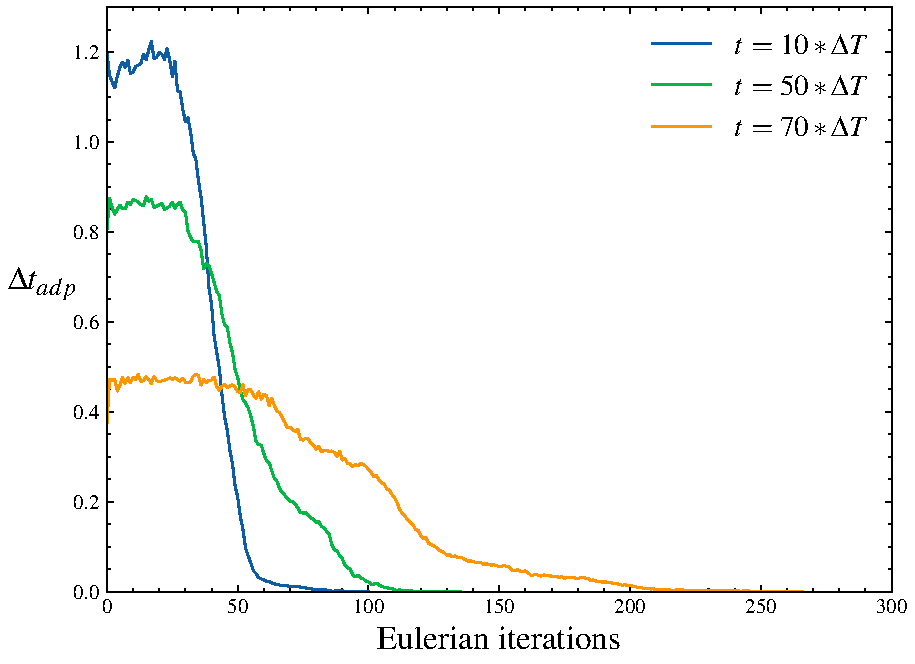
\includegraphics[scale=0.5]{cpc_img/fig_dts1.pdf}
    \caption{The variation of time step $\Delta t_{adp}$ 
     with the number of iterations for Eulerian calculation.  
    %choosen adaptively in different times of the Lagrangian grid. For each Lagrangian-Eulerian time step, hundreds of interactions are carried on Eulerian grid, and the time step is converged to smaller values until reach $\Delta T$. As the system evolves nonlinearly, the iteractions within one step is increasing due to smaller $\Delta t_{adp}$
    }
    \label{fig.adapetive}
\end{figure}
